% !TEX root = ../notes_unsupervisedlearning.tex
% Chapter 3: Hierarchical Clustering
%%%%%%%%%%%%%%%%%%%%%%%%%%%%%%%%%%%%%%%%%%%%%%%%%%%%%%%%%%%%%%%%%%%%%%

\chapter{Hierarchical Clustering}\index{hierarchical clustering}\index{dendrogram}
\newthought{All levels at once.}

% ==============================================================================================
% BLOCK 1: INTRODUCTION
% ==============================================================================================

\newthought{The Why}\index{centroid clustering!limitations}



K-Means left us with three sharp problems.

\newthought{The centroid assumption} forces every cluster to be convex and compact.
A single mean position must stand in for all members, so the algorithm breaks whenever 
clusters are elongated, ring-shaped, or split across multiple densities. All cluster characteristics 
and structure information are lost and filtered when the mean is computed.
The centroid then lands somewhere no data actually lives, and every assignment made 
from that position is wrong by construction.

\newthought{Sensitivity to initialization and outliers} means results are non-deterministic.
A single extreme point can pull a centroid far from the dense mass of its cluster, silently distorting every assignment downstream.
Different random starts can converge to entirely different partitions of the same data.

\newthought{A single scale of structure} is all K-Means can see at once.
With $K{=}2$ you recover two broad groups; with $K{=}10$ you recover ten fine subgroups.
Both are valid descriptions of the same data at different levels of zoom, yet K-Means forces you to choose one and discard the other.
This is not a flaw in the algorithm but a flaw in the question: asking ``how many clusters?'' presupposes that data has one natural scale.

\begin{marginfigure}
    \centering
    \begin{tikzpicture}
        \begin{axis}[
            xmin=0, xmax=10, ymin=0, ymax=10,
            width=\marginparwidth, height=\marginparwidth,
            axis line style={draw=none},
            tick style={black, thin},
            xtick={1,3,5,7,9}, ytick={1,3,5,7,9},
            xticklabel style={font=\tiny},
            yticklabel style={font=\tiny},
            tick align=outside, tick pos=left,
        ]
        % Dotted lines from mu1=(2,2) to C1 points
        \addplot[dotted, black, thin] coordinates {(2,2)(1,2)};
        \addplot[dotted, black, thin] coordinates {(2,2)(2,3)};
        \addplot[dotted, black, thin] coordinates {(2,2)(3,1)};
        % Dotted lines from mu2=(7.33,8) to C2 points
        \addplot[dotted, black!55, thin] coordinates {(7.33,8)(6,8)};
        \addplot[dotted, black!55, thin] coordinates {(7.33,8)(8,7)};
        \addplot[dotted, black!55, thin] coordinates {(7.33,8)(8,9)};
        % Data points
        \addplot[only marks, mark=*, mark size=2pt, black] coordinates {(1,2)(2,3)(3,1)};
        \addplot[only marks, mark=*, mark size=2pt, black!55] coordinates {(6,8)(8,7)(8,9)};
        % Centroids
        \addplot[only marks, mark=o, mark size=2pt, black, thick] coordinates {(2,2)};
        \addplot[only marks, mark=o, mark size=2pt, black!55, thick] coordinates {(7.33,8)};
        \node[font=\tiny, anchor=south east] at (axis cs:1,2) {$x_1$};
        \node[font=\tiny, anchor=south east] at (axis cs:2,3) {$x_2$};
        \node[font=\tiny, anchor=north]      at (axis cs:3,1) {$x_3$};
        \node[font=\tiny, anchor=south west] at (axis cs:6,8) {$x_4$};
        \node[font=\tiny, anchor=north west] at (axis cs:8,7) {$x_5$};
        \node[font=\tiny, anchor=south west] at (axis cs:8,9) {$x_6$};
        \node[font=\tiny, anchor=north east] at (axis cs:2,2) {$\mu_1$};
        \node[font=\tiny, anchor=north]      at (axis cs:7.33,8) {$\mu_2$};
        \end{axis}
    \end{tikzpicture}
    \caption{The canonical six points in two natural clusters $K=2$. Open circles mark the centroids $\mu_1{=}(2,2)$ and $\mu_2{\approx}(7.3,8)$; dotted lines show the distance each point contributes to inertia.}
    \label{fig:why_canonical}
    \end{marginfigure}

\newthought{Hierarchy is the natural answer.} Structure in real data rarely lives at a single scale.
Biological taxonomy nests species inside genera inside families inside orders.
A document corpus organizes words into topics and topics into domains.
File systems nest folders inside folders.
In each case, the right question is not ``how many clusters?'' but ``which level of abstraction do I need right now?''.



\newthought{Hierarchical clustering} produces a dendrogram\index{dendrogram}: a binary tree in 
which leaves are individual data points and each internal node records the distance at 
which two sub-trees were merged.
The full range of partitions, from $K{=}1$ to $K{=}n$, lives in this one structure.

\marginnote{\newthought{The same distance matrix} that K-Means uses to assign points to centroids can be 
used to build an entire tree of clusterings. The tree is built in one pass; 
every value of $K$ is then available for free.}

\newthought{In order to move from a flat partition to a full hierarchy} of clusterings, we have good reason to find ways to,
\begin{itemize}
    \item extend pairwise point distances to cluster distances, making the notion of closest pair well-defined at every scale.
    \item record each merge in a tree structure that makes every partition from $K{=}1$ to $K{=}n$ readable in a single pass.
    \item understand how the choice of cluster distance and linkage design shapes the resulting hierarchy and where it fails.
\end{itemize}





\newpage
\subsection{Hands-On Experience}
\marginnote{\newthought{Divisive clustering}\index{divisive clustering} (top-down) starts with all points in one cluster and recursively splits the cluster with the largest diameter. It is rarely used in practice: splitting is more expensive than merging, and early splits made with global information can be noisier than local merges.}

\newthought{How would you build a hierarchy} of clusterings over these six points?
Which is the cluster on the highest level of abstraction, $K{=}1$? 
How easy is it to build hierarchy top down? Which are the two clusters on the 
second highest level, $K{=}2$? Still obvious, then it gets trickier 
when $K{=}3$ the first non-trivial design-choices are to be made.

\vspace{1.5em}

\begin{figure}
\centering
\begin{tikzpicture}[scale=1]
    \begin{axis}[
        xmin=0, xmax=10,
        ymin=0, ymax=10,
        width=0.5\textwidth,
        height=0.5\textwidth,
        axis line style={draw=none},
        tick style={black, thick},
        xtick={1,2,3,4,5,6,7,8,9},
        ytick={1,2,3,4,5,6,7,8,9},
        xticklabel style={font=\small},
        yticklabel style={font=\small},
        tick align=outside,
        tick pos=left,
    ]
    \addplot[only marks, mark=*, mark size=2pt, black] coordinates {
        (1,2) (2,3) (3,1)
    };
    \addplot[only marks, mark=*, mark size=2pt, black!55] coordinates {
        (6,8) (8,7) (8,9)
    };
    \node[font=\small, anchor=south east] at (axis cs:1,2) {$x_1$};
    \node[font=\small, anchor=south east] at (axis cs:2,3) {$x_2$};
    \node[font=\small, anchor=north]      at (axis cs:3,1) {$x_3$};
    \node[font=\small, anchor=south west] at (axis cs:6,8) {$x_4$};
    \node[font=\small, anchor=north west] at (axis cs:8,7) {$x_5$};
    \node[font=\small, anchor=south west] at (axis cs:8,9) {$x_6$};
    \end{axis}
\end{tikzpicture}
\caption{The canonical six points. Which two are closest? Try building a hierarchy top-down, then bottom-up, which one is easier?}
\label{fig:hc_intro_scatter}
\end{figure}



\newthought{Building Hierarchy Bottom Up} is more intuitive. 
Which points are closest to each other?
See how this again draws on our understanding of distance as a proxy for similarity?
Connect them with a line.
Now find the next closest pair and connect them.
Keep going until all six points are linked into a tree.
At what level of distance would you cut that tree to recover two groups? Three groups?
\marginnote{\newthought{A horizontal cut} at any chosen height yields a flat partition, as we are used to as a result of K-Means.}

\vspace{0.5em}

\newthought{The fundamental question} this chapter answers is how do we formalize
the bottom-up merging process?
We will see how agglomerative clustering builds a dendrogram from pairwise distances;
and how different linkage criteria encode different assumptions about what makes two clusters close.
\marginnote{\newthought{Linkage, is non-trivial.} Two points intuitively merge into a cluster, but beyond that we need a rule for measuring the distance from that cluster to everything else. Do we use the closest pair of points across the two clusters? The furthest? The average? Each answer is a different linkage criterion, and each one tells a different story about what ``nearby clusters'' means.}

\newthought{The Learning Objectives} of this lecture:
\begin{itemize}
    \item Understand how agglomerative clustering builds a dendrogram through successive minimum-distance merges, and read merge-height gaps to identify the natural number of clusters.
    \item Apply single, complete, and Ward's linkage and explain how each criterion shapes the resulting hierarchy.
    \item Identify when hierarchical clustering succeeds where K-Means fails, recognise its failure modes, and explain why scalability requires approximations such as BIRCH.
\end{itemize}










% ==============================================================================================
% BLOCK 2: MAIN THEORY
% ==============================================================================================

\newpage

\subsection{The Hierarchical Clustering Algorithm}\index{agglomerative clustering}

\newthought{The agglomerative strategy}\index{agglomerative clustering}\cite{Ward1963} is bottom-up: given data $X = \{x_1,\ldots,x_n\}$, initialize $n$ singleton clusters $C_i = \{x_i\}$ in an active set and precompute a distance matrix $D[i,j] = d(x_i, x_j)$.
At each step the closest pair $(i^*,j^*) = \arg\min_{i \neq j} D[i,j]$ is merged into $C_m = C_{i^*} \cup C_{j^*}$; the distances to remaining active clusters are updated via linkage criterion $L$.
Every merge is recorded as an internal node of the dendrogram $T$, labeled with the distance $D[i^*,j^*]$ at which it occurred.

\newthought{The result} $T$ is a binary tree.
Every valid flat partition from $K{=}1$ to $K{=}n$ can be read off by making a horizontal cut at the desired height.
The $n-1$ merge heights span the full range from the smallest pairwise distance to the diameter of the data.

\vspace{2.5em}
\begin{algorithm}[H]
\caption{Agglomerative Hierarchical Clustering. }
\begin{algorithmic}[1]
\Require Data $X = \{x_1, \ldots, x_n\}$, linkage criterion $L$
\Ensure Dendrogram $T$
\State Initialize: $C_i \gets \{x_i\}$ for $i = 1,\ldots,n$; active $\gets \{C_1,\ldots,C_n\}$
\State Compute $D[i,j] \gets d(x_i, x_j)$ for all $i \neq j$
\While{$\lvert\mathrm{active}\rvert > 1$}
    \State $(i^*,\;j^*) \gets \arg\min_{i \neq j}\; D[i,j]$
    \State \textbf{Record merge:} $\bigl(C_{i^*},\, C_{j^*}\bigr)$ at height $D[i^*,j^*]$ in $T$
    \State $C_m \gets C_{i^*} \cup C_{j^*}$
    \State Update $D[m,\,k] \gets L(C_m,\,C_k)$ for each active $C_k \neq C_{i^*},C_{j^*}$
    \State Remove $C_{i^*}$ and $C_{j^*}$ from active; add $C_m$
\EndWhile
\end{algorithmic}
\end{algorithm}

\newthought{Notice that $L$ is the only design choice.} 
The algorithm is otherwise fully deterministic. 

\newthought{Initialization is deterministic.} Each point starts as its own singleton cluster,
there is nothing to choose. This stands in sharp contrast to $k$-means, 
where a random centroid draw forces multiple restarts for optimization. Here, the starting state 
is uniquely determined by the data, so two runs on the same dataset always produce the same 
dendrogram.

\newthought{Trace through our six points.} Dotted edges represent pairwise distance calculations;
the dashed edge marks the current merge; gray edges record prior ones.



\begin{figure}
\centering
\begin{tikzpicture}
    \begin{axis}[
        xlabel={$x^{(1)}$}, ylabel={$x^{(2)}$},
        xmin=0, xmax=10, ymin=0, ymax=10,
        width=0.5\textwidth, height=0.5\textwidth,
        axis line style={draw=none},
        tick style={black, thin},
        xtick={2,4,6,8}, ytick={2,4,6,8},
        xticklabel style={font=\small},
        yticklabel style={font=\small},
        tick align=outside, tick pos=left,
    ]
    \addplot[only marks, mark=*, mark size=2pt, black] coordinates {(1,2)(2,3)(3,1)(6,8)(8,7)(8,9)};
    \node[font=\tiny, anchor=north west] at (axis cs:1.1,1.8) {$x_1, C_1$};
    \node[font=\tiny, anchor=south west] at (axis cs:2.1,3) {$x_2, C_2$};
    \node[font=\tiny, anchor=north] at (axis cs:3,0.8) {$x_3, C_3$};
    \node[font=\tiny, anchor=south] at (axis cs:6,8.2) {$x_4, C_4$};
    \node[font=\tiny, anchor=north east] at (axis cs:8,7) {$x_5, C_5$};
    \node[font=\tiny, anchor=south east] at (axis cs:8,9) {$x_6, C_6$};
    \end{axis}
\end{tikzpicture}
\caption{\newthought{Initialization}: $n{=}6$ singleton clusters $C_i{=}\{x_i\}$ placed in the active set.}
\label{fig:hclust_init}
\end{figure}

\begin{figure}
\centering
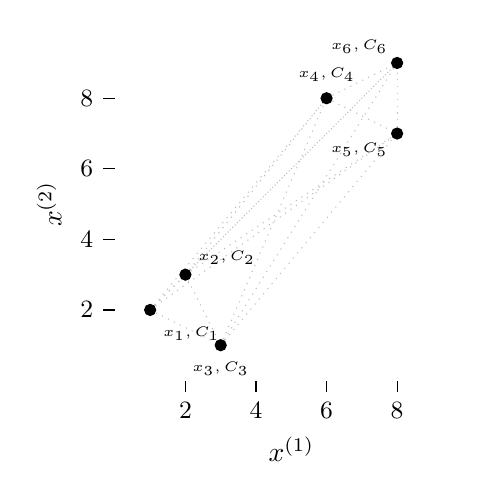
\begin{tikzpicture}
    \begin{axis}[
        xlabel={$x^{(1)}$}, ylabel={$x^{(2)}$},
        xmin=0, xmax=10, ymin=0, ymax=10,
        width=0.5\textwidth, height=0.5\textwidth,
        axis line style={draw=none},
        tick style={black, thin},
        xtick={2,4,6,8}, ytick={2,4,6,8},
        xticklabel style={font=\small},
        yticklabel style={font=\small},
        tick align=outside, tick pos=left,
    ]
    % all 15 pairwise edges
    \draw[black!25, dotted, thin] (axis cs:1,2) -- (axis cs:2,3);
    \draw[black!25, dotted, thin] (axis cs:1,2) -- (axis cs:3,1);
    \draw[black!25, dotted, thin] (axis cs:1,2) -- (axis cs:6,8);
    \draw[black!25, dotted, thin] (axis cs:1,2) -- (axis cs:8,7);
    \draw[black!25, dotted, thin] (axis cs:1,2) -- (axis cs:8,9);
    \draw[black!25, dotted, thin] (axis cs:2,3) -- (axis cs:3,1);
    \draw[black!25, dotted, thin] (axis cs:2,3) -- (axis cs:6,8);
    \draw[black!25, dotted, thin] (axis cs:2,3) -- (axis cs:8,7);
    \draw[black!25, dotted, thin] (axis cs:2,3) -- (axis cs:8,9);
    \draw[black!25, dotted, thin] (axis cs:3,1) -- (axis cs:6,8);
    \draw[black!25, dotted, thin] (axis cs:3,1) -- (axis cs:8,7);
    \draw[black!25, dotted, thin] (axis cs:3,1) -- (axis cs:8,9);
    \draw[black!25, dotted, thin] (axis cs:6,8) -- (axis cs:8,7);
    \draw[black!25, dotted, thin] (axis cs:6,8) -- (axis cs:8,9);
    \draw[black!25, dotted, thin] (axis cs:8,7) -- (axis cs:8,9);
    \addplot[only marks, mark=*, mark size=2pt, black] coordinates {(1,2)(2,3)(3,1)(6,8)(8,7)(8,9)};
    \node[font=\tiny, anchor=north west] at (axis cs:1.1,1.8) {$x_1, C_1$};
    \node[font=\tiny, anchor=south west] at (axis cs:2.1,3) {$x_2, C_2$};
    \node[font=\tiny, anchor=north] at (axis cs:3,0.8) {$x_3, C_3$};
    \node[font=\tiny, anchor=south] at (axis cs:6,8.2) {$x_4, C_4$};
    \node[font=\tiny, anchor=north east] at (axis cs:8,7) {$x_5, C_5$};
    \node[font=\tiny, anchor=south east] at (axis cs:8,9) {$x_6, C_6$};
    \end{axis}
\end{tikzpicture}
\caption{\newthought{Compute} $D[i,j]{=}d(x_i,x_j)$ for all $\binom{6}{2}{=}15$ pairs. 
Each dotted edge is one entry in the distance matrix. 
At every iteration the algorithm selects the globally shortest edge,
 $(i^*,j^*) = \arg\min_{i \neq j}\, D[i,j]$, where $i,j$ range only over the current active set. Once $C_{i^*}$ and $C_{j^*}$ are merged into $C_m$, they are removed from active and replaced by $C_m$; past merges are never revisited.}
\label{fig:hclust_distances}
\end{figure}


\begin{figure}
\centering
\begin{tikzpicture}
    \begin{axis}[
        xlabel={$x^{(1)}$}, ylabel={$x^{(2)}$},
        xmin=0, xmax=10, ymin=0, ymax=10,
        width=0.5\textwidth, height=0.5\textwidth,
        axis line style={draw=none},
        tick style={black, thin},
        xtick={2,4,6,8}, ytick={2,4,6,8},
        xticklabel style={font=\small},
        yticklabel style={font=\small},
        tick align=outside, tick pos=left,
    ]
    \addplot[only marks, mark=*, mark size=2pt, black] coordinates {(1,2)(2,3)(3,1)(6,8)(8,7)(8,9)};
    \draw[black!55, densely dashed] (axis cs:1,2) -- (axis cs:2,3);
    \node[font=\tiny, anchor=north west] at (axis cs:1.1,1.8) {$x_1, C_m$};
    \node[font=\tiny, anchor=south west] at (axis cs:2.1,3) {$x_2, C_m$};
    \node[font=\tiny, anchor=north] at (axis cs:3,0.8) {$x_3, C_3$};
    \node[font=\tiny, anchor=south] at (axis cs:6,8.2) {$x_4, C_4$};
    \node[font=\tiny, anchor=north east] at (axis cs:8,7) {$x_5, C_5$};
    \node[font=\tiny, anchor=south east] at (axis cs:8,9) {$x_6, C_6$};
    \end{axis}
\end{tikzpicture}
\caption{\newthought{Merge 1}: the globally smallest distance is $d(x_1,x_2)$. 
Singletons $\{x_1\}$ and $\{x_2\}$ merge into $C_m{=}\{x_1,x_2\}$, 
recorded as an internal node in $T$ with both singletons as children, 
labeled by $d(x_1,x_2)$: $T \mathrel{+}= C_7 = \bigl(C_1,\, C_2,\, d(x_1,x_2)\bigr)$.}
\label{fig:hclust_merge1}
\end{figure}


\begin{figure}
\centering
\begin{tikzpicture}
    \begin{axis}[
        xlabel={$x^{(1)}$}, ylabel={$x^{(2)}$},
        xmin=0, xmax=10, ymin=0, ymax=10,
        width=0.5\textwidth, height=0.5\textwidth,
        axis line style={draw=none},
        tick style={black, thin},
        xtick={2,4,6,8}, ytick={2,4,6,8},
        xticklabel style={font=\small},
        yticklabel style={font=\small},
        tick align=outside, tick pos=left,
    ]
    \addplot[only marks, mark=*, mark size=2pt, black] coordinates {(1,2)(2,3)(3,1)(6,8)(8,7)(8,9)};
    \draw[black!35, thin] (axis cs:1,2) -- (axis cs:2,3);
    % new D entries: C_m to remaining singletons, nearest member under single linkage
    \draw[black!25, dotted, thin] (axis cs:2,3) -- (axis cs:3,1);
    \draw[black!25, dotted, thin] (axis cs:2,3) -- (axis cs:6,8);
    \draw[black!25, dotted, thin] (axis cs:2,3) -- (axis cs:8,7);
    \draw[black!25, dotted, thin] (axis cs:2,3) -- (axis cs:8,9);
    \node[font=\tiny, anchor=north west] at (axis cs:1.1,1.8) {$x_1, C_m$};
    \node[font=\tiny, anchor=south west] at (axis cs:2.1,3) {$x_2, C_m$};
    \node[font=\tiny, anchor=north] at (axis cs:3,0.8) {$x_3, C_3$};
    \node[font=\tiny, anchor=south] at (axis cs:6,8.2) {$x_4, C_4$};
    \node[font=\tiny, anchor=north east] at (axis cs:8,7) {$x_5, C_5$};
    \node[font=\tiny, anchor=south east] at (axis cs:8,9) {$x_6, C_6$};
    \end{axis}
\end{tikzpicture}
\caption{\newthought{Update $D$}: after forming $C_7{=}\{x_1,x_2\}$, four rows and columns 
of $D$ are refreshed via $D[7,k] \gets L(C_7, C_k)$. Under single linkage $L$ takes 
the nearest member: $D[7,k] = \min_{x \in C_7}\, d(x, C_k)$. 
Here $x_2$ is the nearest member of $C_7$ to all remaining singletons, 
so every new entry anchors at $x_2$ (dotted edges).

\newthought{Discuss Linkage}}
\label{fig:hclust_update1}
\end{figure}

\begin{figure}
\centering
\begin{tikzpicture}
    \begin{axis}[
        xlabel={$x^{(1)}$}, ylabel={$x^{(2)}$},
        xmin=0, xmax=10, ymin=0, ymax=10,
        width=0.5\textwidth, height=0.5\textwidth,
        axis line style={draw=none},
        tick style={black, thin},
        xtick={2,4,6,8}, ytick={2,4,6,8},
        xticklabel style={font=\small},
        yticklabel style={font=\small},
        tick align=outside, tick pos=left,
    ]
    \addplot[only marks, mark=*, mark size=2pt, black] coordinates {(1,2)(2,3)(3,1)(6,8)(8,7)(8,9)};
    \draw[black!35, thin] (axis cs:1,2) -- (axis cs:2,3);
    \draw[black!55, densely dashed] (axis cs:8,7) -- (axis cs:8,9);
    \node[font=\tiny, anchor=north west] at (axis cs:1.1,1.8) {$x_1, C_7$};
    \node[font=\tiny, anchor=south west] at (axis cs:2.1,3) {$x_2, C_7$};
    \node[font=\tiny, anchor=north] at (axis cs:3,0.8) {$x_3, C_3$};
    \node[font=\tiny, anchor=south] at (axis cs:6,8.2) {$x_4, C_4$};
    \node[font=\tiny, anchor=north east] at (axis cs:8,7) {$x_5, C_m$};
    \node[font=\tiny, anchor=south east] at (axis cs:8,9) {$x_6, C_m$};
    \end{axis}
\end{tikzpicture}
\caption{\newthought{Merge 2}: the next minimum in the updated $D$ is $d(x_5,x_6)$. Singletons $\{x_5\}$ and $\{x_6\}$ merge into $C_m{=}\{x_5,x_6\}$, recorded in $T$ as $T \mathrel{+}= C_8 = \bigl(C_5,\, C_6,\, d(x_5,x_6)\bigr)$.}
\label{fig:hclust_merge2}
\end{figure}

\begin{figure}
\centering
\begin{tikzpicture}
    \begin{axis}[
        xlabel={$x^{(1)}$}, ylabel={$x^{(2)}$},
        xmin=0, xmax=10, ymin=0, ymax=10,
        width=0.5\textwidth, height=0.5\textwidth,
        axis line style={draw=none},
        tick style={black, thin},
        xtick={2,4,6,8}, ytick={2,4,6,8},
        xticklabel style={font=\small},
        yticklabel style={font=\small},
        tick align=outside, tick pos=left,
    ]
    \addplot[only marks, mark=*, mark size=2pt, black] coordinates {(1,2)(2,3)(3,1)(6,8)(8,7)(8,9)};
    \draw[black!35, thin] (axis cs:1,2) -- (axis cs:2,3);
    \draw[black!35, thin] (axis cs:8,7) -- (axis cs:8,9);
    \draw[black!55, densely dashed] (axis cs:6,8) -- (axis cs:8,7);
    \node[font=\tiny, anchor=north west] at (axis cs:1.1,1.8) {$x_1, C_7$};
    \node[font=\tiny, anchor=south west] at (axis cs:2.1,3) {$x_2, C_7$};
    \node[font=\tiny, anchor=north] at (axis cs:3,0.8) {$x_3, C_3$};
    \node[font=\tiny, anchor=south] at (axis cs:6,8.2) {$x_4, C_m$};
    \node[font=\tiny, anchor=north east] at (axis cs:8,7) {$x_5, C_m$};
    \node[font=\tiny, anchor=south east] at (axis cs:8,9) {$x_6, C_m$};
    \end{axis}
\end{tikzpicture}
\caption{\newthought{Merge 3}: $D\bigl(C_8,x_4\bigr)$ is minimal under single linkage (distances to a merged cluster use the nearest member). $D\bigl(C_7,x_3\bigr)$ ties but $x_4$ merges first by index. Cluster $C_8$ absorbs $x_4$, linking via $x_5$: $T \mathrel{+}= C_9 = \bigl(C_8,\, C_4,\, D(C_8, C_4)\bigr)$.}
\label{fig:hclust_merge3}
\end{figure}

\begin{figure}
\centering
\begin{tikzpicture}
    \begin{axis}[
        xlabel={$x^{(1)}$}, ylabel={$x^{(2)}$},
        xmin=0, xmax=10, ymin=0, ymax=10,
        width=0.5\textwidth, height=0.5\textwidth,
        axis line style={draw=none},
        tick style={black, thin},
        xtick={2,4,6,8}, ytick={2,4,6,8},
        xticklabel style={font=\small},
        yticklabel style={font=\small},
        tick align=outside, tick pos=left,
    ]
    \addplot[only marks, mark=*, mark size=2pt, black] coordinates {(1,2)(2,3)(3,1)(6,8)(8,7)(8,9)};
    \draw[black!35, thin] (axis cs:1,2) -- (axis cs:2,3);
    \draw[black!35, thin] (axis cs:8,7) -- (axis cs:8,9);
    \draw[black!35, thin] (axis cs:6,8) -- (axis cs:8,7);
    \draw[black!55, densely dashed] (axis cs:2,3) -- (axis cs:3,1);
    \node[font=\tiny, anchor=north west] at (axis cs:1.1,1.8) {$x_1, C_m$};
    \node[font=\tiny, anchor=south west] at (axis cs:2.1,3) {$x_2, C_m$};
    \node[font=\tiny, anchor=north] at (axis cs:3,0.8) {$x_3, C_m$};
    \node[font=\tiny, anchor=south] at (axis cs:6,8.2) {$x_4, C_9$};
    \node[font=\tiny, anchor=north east] at (axis cs:8,7) {$x_5, C_9$};
    \node[font=\tiny, anchor=south east] at (axis cs:8,9) {$x_6, C_9$};
    \end{axis}
\end{tikzpicture}
\caption{\newthought{Merge 4}: also at height $\sqrt{5}$, $D\bigl(C_7,x_3\bigr)=\sqrt{5}$. Cluster $C_7$ absorbs $x_3$, linking via $x_2$: $T \mathrel{+}= C_{10} = \bigl(C_7,\, C_3,\, D(C_7, C_3)\bigr)$.}
\label{fig:hclust_merge4}
\end{figure}

\begin{figure}
\centering
\begin{tikzpicture}
    \begin{axis}[
        xlabel={$x^{(1)}$}, ylabel={$x^{(2)}$},
        xmin=0, xmax=10, ymin=0, ymax=10,
        width=0.5\textwidth, height=0.5\textwidth,
        axis line style={draw=none},
        tick style={black, thin},
        xtick={2,4,6,8}, ytick={2,4,6,8},
        xticklabel style={font=\small},
        yticklabel style={font=\small},
        tick align=outside, tick pos=left,
    ]
    \addplot[only marks, mark=*, mark size=2pt, black] coordinates {(1,2)(2,3)(3,1)(6,8)(8,7)(8,9)};
    \draw[black!35, thin] (axis cs:1,2) -- (axis cs:2,3);
    \draw[black!35, thin] (axis cs:8,7) -- (axis cs:8,9);
    \draw[black!35, thin] (axis cs:6,8) -- (axis cs:8,7);
    \draw[black!35, thin] (axis cs:2,3) -- (axis cs:3,1);
    \draw[black!55, densely dashed] (axis cs:2,3) -- (axis cs:6,8);
    \node[font=\tiny, anchor=north west] at (axis cs:1.1,1.8) {$x_1, C_{m}$};
    \node[font=\tiny, anchor=south west] at (axis cs:2.1,3) {$x_2, C_{m}$};
    \node[font=\tiny, anchor=north] at (axis cs:3,0.8) {$x_3, C_{m}$};
    \node[font=\tiny, anchor=south] at (axis cs:6,8.2) {$x_4, C_m$};
    \node[font=\tiny, anchor=north east] at (axis cs:8,7) {$x_5, C_m$};
    \node[font=\tiny, anchor=south east] at (axis cs:8,9) {$x_6, C_m$};
    \end{axis}
\end{tikzpicture}
\caption{\newthought{Merge 5}: $C_{10}{=}\{x_1,x_2,x_3\}$ and $C_9{=}\{x_4,x_5,x_6\}$ merge at height $d(x_2,x_4)$, the nearest cross-cluster pair. All six points form one cluster; the dendrogram $T$ is complete.}
\label{fig:hclust_merge5}
\end{figure}

\begin{figure}
\centering
\begin{tikzpicture}
    \begin{axis}[
        xlabel={$x^{(1)}$}, ylabel={$x^{(2)}$},
        xmin=0, xmax=10, ymin=0, ymax=10,
        width=0.5\textwidth, height=0.5\textwidth,
        axis line style={draw=none},
        tick style={black, thin},
        xtick={2,4,6,8}, ytick={2,4,6,8},
        xticklabel style={font=\small},
        yticklabel style={font=\small},
        tick align=outside, tick pos=left,
    ]
    \addplot[only marks, mark=*, mark size=2pt, black] coordinates {(1,2)(2,3)(3,1)(6,8)(8,7)(8,9)};
    \draw[black!35, thin] (axis cs:1,2) -- (axis cs:2,3);
    \draw[black!35, thin] (axis cs:8,7) -- (axis cs:8,9);
    \draw[black!35, thin] (axis cs:6,8) -- (axis cs:8,7);
    \draw[black!35, thin] (axis cs:2,3) -- (axis cs:3,1);
    \draw[black!35, thin] (axis cs:2,3) -- (axis cs:6,8);
    \node[font=\tiny, anchor=north west] at (axis cs:1.1,1.8) {$x_1, C_{11}$};
    \node[font=\tiny, anchor=south west] at (axis cs:2.1,3) {$x_2, C_{11}$};
    \node[font=\tiny, anchor=north] at (axis cs:3,0.8) {$x_3, C_{11}$};
    \node[font=\tiny, anchor=south] at (axis cs:6,8.2) {$x_4, C_{11}$};
    \node[font=\tiny, anchor=north east] at (axis cs:8,7) {$x_5, C_{11}$};
    \node[font=\tiny, anchor=south east] at (axis cs:8,9) {$x_6, C_{11}$};
    \end{axis}
\end{tikzpicture}
\caption{\newthought{Termination:} $|\mathrm{active}|{=}1$. All $n{=}6$ points belong to $C_{11}$; the five merge edges span the complete single-linkage dendrogram. No further merges are possible.}
\label{fig:hclust_terminate}
\end{figure}





\marginnote{\newthought{Remove Two. Add One.} In every 
iteration reduces $|\mathrm{active}|$ by exactly one 
(two clusters are removed and one merged cluster is added)}
\newthought{Termination.} The algorithm halts when $|\mathrm{active}| = 1$: exactly one 
cluster remains, containing all $n$ points. Termination is guaranteed after exactly $n-1$ merges. At that point $T$ holds $n-1$ internal nodes, 
one per merge, and is the complete dendrogram.








\vspace{2.5em}
\marginnote{\newthought{Answers from where we measure the distance.} The distance then still decides what we are going to merge.}

\newthought{Linkage criteria beyond two points is non-trivial}\index{linkage criterion} 
determine how the distance between two clusters is computed from the distances between 
their individual members.
The choice of linkage profoundly shapes the dendrogram. Swap $L$ and you get a fundamentally 
different clustering.



\newthought{Single Linkage}\index{single linkage}

\begin{align*}
    D_{\mathrm{single}}(C_i,\, C_j) &= \min_{x \in C_i,\; y \in C_j} d(x,\, y)
\end{align*}

\begin{marginfigure}
\centering
\begin{tikzpicture}
    \begin{axis}[
        xmin=0, xmax=10, ymin=0, ymax=10,
        width=\marginparwidth, height=\marginparwidth,
        axis line style={draw=none},
        tick style={black, thin},
        xtick={1,3,5,7,9}, ytick={1,3,5,7,9},
        xticklabel style={font=\tiny},
        yticklabel style={font=\tiny},
        tick align=outside, tick pos=left,
    ]
    % C_7={x1,x2} dark; C_8={x5,x6} gray; singletons x3,x4 light
    \addplot[only marks, mark=*, mark size=2pt, black]    coordinates {(1,2)(2,3)};
    \addplot[only marks, mark=*, mark size=2pt, black!55] coordinates {(8,7)(8,9)};
    \addplot[only marks, mark=*, mark size=2pt, black!30] coordinates {(3,1)(6,8)};
    \draw[black!35, thin] (axis cs:1,2) -- (axis cs:2,3);
    \draw[black!35, thin] (axis cs:8,7) -- (axis cs:8,9);
    % Single linkage: nearest member per cluster pair (dotted)
    \draw[black!30, dotted, thin] (axis cs:2,3) -- (axis cs:3,1);  % C_7--C_3
    \draw[black!30, dotted, thin] (axis cs:2,3) -- (axis cs:6,8);  % C_7--C_4
    \draw[black!30, dotted, thin] (axis cs:2,3) -- (axis cs:8,7);  % C_7--C_8
    \draw[black!30, dotted, thin] (axis cs:3,1) -- (axis cs:6,8);  % C_3--C_4
    \draw[black!30, dotted, thin] (axis cs:3,1) -- (axis cs:8,7);  % C_3--C_8
    \draw[black!30, dotted, thin] (axis cs:6,8) -- (axis cs:8,7);  % C_4--C_8
    \node[font=\tiny, anchor=north west] at (axis cs:1.1,1.8) {$x_1$};
    \node[font=\tiny, anchor=south east] at (axis cs:2,3)     {$x_2$};
    \node[font=\tiny, anchor=north]      at (axis cs:3,1)     {$x_3$};
    \node[font=\tiny, anchor=south west] at (axis cs:6,8)     {$x_4$};
    \node[font=\tiny, anchor=north west] at (axis cs:8,7)     {$x_5$};
    \node[font=\tiny, anchor=south west] at (axis cs:8,9)     {$x_6$};
    \end{axis}
\end{tikzpicture}
\caption{Single linkage: dotted lines show $d_{\min}$ for each of the six active cluster pairs. The smallest, $d(x_2,x_3){=}d(x_4,x_5)$, determines the next merge.}
\label{fig:linkage_single}
\end{marginfigure}


The distance between two clusters is the distance between their nearest members.
Single linkage admits an implementation based on Prim's minimal spanning tree (details later), which is fast. This also lets it detect elongated, 
non-convex clusters. This behavior is called chaining, and is also a weakness; a single close pair of 
points can bridge two otherwise distant clusters, pulling them into one.

\newthought{Complete Linkage}\index{complete linkage}

\begin{align*}
    D_{\mathrm{complete}}(C_i,\, C_j) &= \max_{x \in C_i,\; y \in C_j} d(x,\, y)
\end{align*}

\begin{marginfigure}
\centering
\begin{tikzpicture}
    \begin{axis}[
        xmin=0, xmax=10, ymin=0, ymax=10,
        width=\marginparwidth, height=\marginparwidth,
        axis line style={draw=none},
        tick style={black, thin},
        xtick={1,3,5,7,9}, ytick={1,3,5,7,9},
        xticklabel style={font=\tiny},
        yticklabel style={font=\tiny},
        tick align=outside, tick pos=left,
    ]
    % C_7={x1,x2} dark; C_8={x5,x6} gray; singletons x3,x4 light
    \addplot[only marks, mark=*, mark size=2pt, black]    coordinates {(1,2)(2,3)};
    \addplot[only marks, mark=*, mark size=2pt, black!55] coordinates {(8,7)(8,9)};
    \addplot[only marks, mark=*, mark size=2pt, black!30] coordinates {(3,1)(6,8)};
    \draw[black!35, thin] (axis cs:1,2) -- (axis cs:2,3);
    \draw[black!35, thin] (axis cs:8,7) -- (axis cs:8,9);
    % Complete linkage: furthest member per cluster pair (dotted)
    \draw[black!30, dotted, thin] (axis cs:1,2)  -- (axis cs:3,1);  % C_7--C_3
    \draw[black!30, dotted, thin] (axis cs:1,2)  -- (axis cs:6,8);  % C_7--C_4
    \draw[black!30, dotted, thin] (axis cs:1,2)  -- (axis cs:8,9);  % C_7--C_8
    \draw[black!30, dotted, thin] (axis cs:3,1)  -- (axis cs:6,8);  % C_3--C_4
    \draw[black!30, dotted, thin] (axis cs:3,1)  -- (axis cs:8,9);  % C_3--C_8
    \draw[black!30, dotted, thin] (axis cs:6,8)  -- (axis cs:8,9);  % C_4--C_8
    \node[font=\tiny, anchor=north west] at (axis cs:1.1,1.8) {$x_1$};
    \node[font=\tiny, anchor=south east] at (axis cs:2,3)     {$x_2$};
    \node[font=\tiny, anchor=north]      at (axis cs:3,1)     {$x_3$};
    \node[font=\tiny, anchor=south west] at (axis cs:6,8)     {$x_4$};
    \node[font=\tiny, anchor=north west] at (axis cs:8,7)     {$x_5$};
    \node[font=\tiny, anchor=south west] at (axis cs:8,9)     {$x_6$};
    \end{axis}
\end{tikzpicture}
\caption{Complete linkage: dotted lines show $d_{\max}$ for each active cluster pair. The largest determines which merge is most expensive.}
\label{fig:linkage_complete}
\end{marginfigure}



The distance between two clusters is the distance between their furthest members.
Complete linkage tends to produce compact, roughly equal-diameter clusters and is robust to chaining.
It may, however, split naturally elongated shapes.

\newthought{Average Linkage}\index{average linkage}

\begin{align*}
    D_{\mathrm{average}}(C_i,\, C_j) &= \frac{1}{|C_i|\,|C_j|} \sum_{x \in C_i} \sum_{y \in C_j} d(x,\, y)
\end{align*}
\begin{marginfigure}
\centering
\begin{tikzpicture}
    \begin{axis}[
        xmin=0, xmax=10, ymin=0, ymax=10,
        width=\marginparwidth, height=\marginparwidth,
        axis line style={draw=none},
        tick style={black, thin},
        xtick={1,3,5,7,9}, ytick={1,3,5,7,9},
        xticklabel style={font=\tiny},
        yticklabel style={font=\tiny},
        tick align=outside, tick pos=left,
    ]
    % C_7={x1,x2} dark; C_8={x5,x6} gray; singletons x3,x4 light
    \addplot[only marks, mark=*, mark size=2pt, black]    coordinates {(1,2)(2,3)};
    \addplot[only marks, mark=*, mark size=2pt, black!55] coordinates {(8,7)(8,9)};
    \addplot[only marks, mark=*, mark size=2pt, black!30] coordinates {(3,1)(6,8)};
    \draw[black!35, thin] (axis cs:1,2) -- (axis cs:2,3);
    \draw[black!35, thin] (axis cs:8,7) -- (axis cs:8,9);
    % Average linkage: all pairwise cross-cluster distances (dotted)
    \draw[black!25, dotted, thin] (axis cs:1,2) -- (axis cs:3,1);
    \draw[black!25, dotted, thin] (axis cs:2,3) -- (axis cs:3,1);
    \draw[black!25, dotted, thin] (axis cs:1,2) -- (axis cs:6,8);
    \draw[black!25, dotted, thin] (axis cs:2,3) -- (axis cs:6,8);
    \draw[black!25, dotted, thin] (axis cs:1,2) -- (axis cs:8,7);
    \draw[black!25, dotted, thin] (axis cs:1,2) -- (axis cs:8,9);
    \draw[black!25, dotted, thin] (axis cs:2,3) -- (axis cs:8,7);
    \draw[black!25, dotted, thin] (axis cs:2,3) -- (axis cs:8,9);
    \draw[black!25, dotted, thin] (axis cs:3,1) -- (axis cs:6,8);
    \draw[black!25, dotted, thin] (axis cs:3,1) -- (axis cs:8,7);
    \draw[black!25, dotted, thin] (axis cs:3,1) -- (axis cs:8,9);
    \draw[black!25, dotted, thin] (axis cs:6,8) -- (axis cs:8,7);
    \draw[black!25, dotted, thin] (axis cs:6,8) -- (axis cs:8,9);
    \node[font=\tiny, anchor=north west] at (axis cs:1.1,1.8) {$x_1$};
    \node[font=\tiny, anchor=south east] at (axis cs:2,3)     {$x_2$};
    \node[font=\tiny, anchor=north]      at (axis cs:3,1)     {$x_3$};
    \node[font=\tiny, anchor=south west] at (axis cs:6,8)     {$x_4$};
    \node[font=\tiny, anchor=north west] at (axis cs:8,7)     {$x_5$};
    \node[font=\tiny, anchor=south west] at (axis cs:8,9)     {$x_6$};
    \end{axis}
\end{tikzpicture}
\caption{Average linkage: $D$ averages all pairwise cross-cluster distances. Every dotted line contributes to the mean.}
\label{fig:linkage_average}
\end{marginfigure}


Also known as the Unweighted Pair Group Method with Arithmetic Mean. Is a compromise: 
less prone to chaining than single linkage, less aggressive at squashing elongated clusters 
than complete linkage.
Average linkage averages all cross-cluster pairwise distances.


\newpage
\newthought{Ward's Method}\index{Ward's method}

\begin{marginfigure}
\centering
\begin{tikzpicture}
    \begin{axis}[
        xmin=0, xmax=10, ymin=0, ymax=10,
        width=\marginparwidth, height=\marginparwidth,
        axis line style={draw=none},
        tick style={black, thin},
        xtick={1,3,5,7,9}, ytick={1,3,5,7,9},
        xticklabel style={font=\tiny},
        yticklabel style={font=\tiny},
        tick align=outside, tick pos=left,
    ]
    % C_7={x1,x2} dark; C_8={x5,x6} gray; singletons x3,x4 light
    \addplot[only marks, mark=*, mark size=2pt, black]    coordinates {(1,2)(2,3)};
    \addplot[only marks, mark=*, mark size=2pt, black!55] coordinates {(8,7)(8,9)};
    \addplot[only marks, mark=*, mark size=2pt, black!30] coordinates {(3,1)(6,8)};
    \draw[black!35, thin] (axis cs:1,2) -- (axis cs:2,3);
    \draw[black!35, thin] (axis cs:8,7) -- (axis cs:8,9);
    % Centroids: mu_7=(1.5,2.5), mu_3=x3=(3,1), mu_4=x4=(6,8), mu_8=(8,8)
    \addplot[only marks, mark=o, mark size=2pt, black, thick]    coordinates {(1.5,2.5)};
    \addplot[only marks, mark=o, mark size=2pt, black!60, thick] coordinates {(3,1)(6,8)};
    \addplot[only marks, mark=o, mark size=2pt, black!55, thick] coordinates {(8,8)};
    % Ward: dotted lines between all centroid pairs
    \draw[black!30, dotted, thin] (axis cs:1.5,2.5) -- (axis cs:3,1);
    \draw[black!30, dotted, thin] (axis cs:1.5,2.5) -- (axis cs:6,8);
    \draw[black!30, dotted, thin] (axis cs:1.5,2.5) -- (axis cs:8,8);
    \draw[black!30, dotted, thin] (axis cs:3,1)     -- (axis cs:6,8);
    \draw[black!30, dotted, thin] (axis cs:3,1)     -- (axis cs:8,8);
    \draw[black!30, dotted, thin] (axis cs:6,8)     -- (axis cs:8,8);
    \node[font=\tiny, anchor=north east] at (axis cs:1.5,2.5) {$\mu_7$};
    \node[font=\tiny, anchor=south west] at (axis cs:8,8)     {$\mu_8$};
    \node[font=\tiny, anchor=north west] at (axis cs:1.1,1.8) {$x_1$};
    \node[font=\tiny, anchor=south east] at (axis cs:2,3)     {$x_2$};
    \node[font=\tiny, anchor=north]      at (axis cs:3,1)     {$x_3$};
    \node[font=\tiny, anchor=south west] at (axis cs:6,8)     {$x_4$};
    \node[font=\tiny, anchor=north west] at (axis cs:8,7)     {$x_5$};
    \node[font=\tiny, anchor=south west] at (axis cs:8,9)     {$x_6$};
    \end{axis}
\end{tikzpicture}
\caption{Ward's linkage: dotted lines connect centroids of all active cluster pairs; $D$ is proportional to $\|\mu_i{-}\mu_j\|^2$ weighted by cluster size.}
\label{fig:linkage_ward}
\end{marginfigure}

Ward's criterion merges the two clusters whose union minimises the increase in 
total within-cluster variance:

\begin{align*}
    D_{\mathrm{Ward}}(C_i,\, C_j) &= \frac{|C_i|\,|C_j|}{|C_i| + |C_j|} \left\|\mu_i - \mu_j\right\|^2
\end{align*}

where $\mu_i$ and $\mu_j$ are the centroids of $C_i$ and $C_j$.
Ward's method produces compact, spherical clusters and is closely related to K-Means as 
both minimise within-cluster variance or inertia. Of course this makes Ward share the 
same weaknesses as K-Means. 





\vspace{2.5em}
\newthought{When Hierarchical Clustering Fails}\index{failure modes!hierarchical clustering} the
root cause is that the linkage criterions optimises locally with no global view nor understanding for 
scale. Every point gets clustered at some point in the agglomeration.

\vspace{2.5em}
\marginnote{\newthought{Chaining and bridging}\index{chaining!single linkage}}

\begin{figure}
    \centering
    \begin{tikzpicture}
        \begin{axis}[
            xlabel={$x^{(1)}$}, ylabel={$x^{(2)}$},
            xmin=0, xmax=10, ymin=0, ymax=10,
            width=0.5\textwidth, height=0.4\textwidth,
            axis line style={draw=none},
            tick style={black, thin},
            xtick={2,4,6,8}, ytick={2,4,6,8},
            xticklabel style={font=\small},
            yticklabel style={font=\small},
            tick align=outside, tick pos=left,
        ]
        % Left cluster (dark)
        \addplot[only marks, mark=*, mark size=2pt, black] coordinates {(1,2)(2,3)(3,1)};
        % Bridge point (light)
        \addplot[only marks, mark=*, mark size=2pt, black!25] coordinates {(5,5)};
        % Right cluster (medium grey)
        \addplot[only marks, mark=*, mark size=2pt, black!55] coordinates {(6,8)(8,7)(8,9)};
        % Within-cluster merges (solid)
        \draw[black!35, thin] (axis cs:1,2) -- (axis cs:2,3);
        \draw[black!35, thin] (axis cs:2,3) -- (axis cs:3,1);
        \draw[black!35, thin] (axis cs:8,7) -- (axis cs:8,9);
        \draw[black!35, thin] (axis cs:6,8) -- (axis cs:8,7);
        % Chaining: bridge absorbed into left cluster, then connects to right (dashed)
        \draw[black!55, densely dashed] (axis cs:3,1) -- (axis cs:5,5);
        \draw[black!55, densely dashed] (axis cs:5,5) -- (axis cs:6,8);
        \end{axis}
    \end{tikzpicture}
    \caption{Single-linkage chaining: one intermediate point (light) bridges two well-separated clusters. Within-cluster merges (solid) complete first; single linkage then greedily closes through the bridge (dashed), incorrectly joining both clusters into one.}
    \label{fig:hc_chaining}
\end{figure}

\newthought{Shape Bias}\index{shape bias!Ward's linkage} Ward's linkage inherits K-Means's spherical 
bias exactly. The difference is recovery: K-Means re-assigns points each iteration and 
can partially correct a bad partition. Ward's cannot; the bias compounds irreversibly.

\marginnote{\newthought{Irrecoverability}\index{irrecoverability!hierarchical clustering} is what makes chaining and shape bias genuinely dangerous. A bad merge silently propagates through every subsequent distance update; the only remedy is to restart from scratch.}

\newthought{Irreversible greedy merges and local optima.} At each step the algorithm 
selects the globally optimal merge under the current distance matrix: no local minimum 
trap exists within a single iteration. However, the greedy (no-reassignment) strategy is myopic. 
Once $C_{i^*}$ and $C_{j^*}$ are merged into $C_m$, that decision is permanent; 
no subsequent step can reverse it. A suboptimal early merge propagates through all 
future distance updates via $L$, and the resulting dendrogram may differ substantially 
from the globally optimal hierarchy.


\vspace{2.5em}
\newthought{Computational Complexity}\index{computational complexity!hierarchical clustering} Memory is the hard wall. The distance matrix $D_{i,j}$ requires $O(n^2)$ space.
At $n{=}100{,}000$ that is already $\approx$40\,GB for float32: you either fit it in RAM or the algorithm cannot run.
\marginnote{$D_{i,j}$ has $\tfrac{n(n-1)}{2}$ entries; $O(n^2)$ space.}

\marginnote{\newthought{float32 at scale.} $n{=}10{,}000$ needs $\approx$400\,MB; $n{=}100{,}000$ needs $\approx$40\,GB.}
\vspace{1.0em}
\newthought{Compute is the soft wall.} Even when the matrix fits, filling it costs $O(n^2)$.
The merge steps then scan and update distances after each of the $n{-}1$ merges, adding $O(n^2)$ for optimised linkages or $O(n^3)$ for naive implementations.


\begin{table*}[ht]
\centering
\begin{tabular}{p{0.30\textwidth}p{0.14\textwidth}p{0.40\textwidth}}
    \toprule
    \textbf{Algorithm} & \textbf{Time} & \textbf{Notes} \\
    \midrule
    K-Means (baseline)         & $O(n)$           & $K$, $T$, $d$ treated as constants \\
    Naive agglomerative        & $O(n^3)$         & Recomputes all distances each step \\
    Single linkage (SLINK)     & $O(n^2)$         & Optimal algorithm for single linkage \\
    Average linkage & $O(n^3)$  & Without acceleration \\
    \bottomrule
\end{tabular}
\vspace{2em}
\caption{Complexity of hierarchical clustering variants; K-Means is the linear baseline ($K$, $T$, $d$ constant).
Naive agglomerative is $O(n^3)$: it rescans the full distance matrix at each of the $n{-}1$ merge steps.}
\label{tab:hc_complexity}
\end{table*}


\vspace{2.5em}
\newthought{Single linkage achieves $O(n^2)$}\index{single linkage!complexity} because its update 
rule is a simple minimum, as the minimal distance to a merged cluster is the minimum of the 
distances to its two constituent, deprecated clusters:
\begin{align*}
    d(C_i \cup C_j,\, C_k) &= \min\bigl(d(C_i,C_k),\, d(C_j,C_k)\bigr)
\end{align*}
SLINK\cite{Sibson1973} exploits this as 
each new point requires only a single scan of the current distances; $O(n)$ 
per update step over $n{-}1$ merges gives $O(n^2)$ total time.

\vspace{2.5em}
\newthought{Scalability by Compression}\index{scalability!hierarchical clustering} is regained by
BIRCH\cite{Zhang1996}\index{BIRCH}, which breaks the $O(n^2)$ memory barrier by compressing 
data into a compressed tree in one pass, then running agglomeration on the leaf nodes rather 
than individual points reducing cost. A threshold $T$ controls compression: 
A small $T$ produces many fine-grained 
leaves (accurate but larger tree); a large $T$ merges more points per leaf (faster but coarser). 
Setting $T$ too large can merge points from different true clusters before agglomeration begins.












\newpage
\begin{marginfigure}
    \centering
    \begin{tikzpicture}
        \begin{axis}[
            xmin=0, xmax=10,
            ymin=0, ymax=10,
            width=\marginparwidth,
            height=\marginparwidth,
            axis line style={draw=none},
            tick style={black, thin},
            xtick={0,3,6,9},
            ytick={0,3,6,9},
            xticklabel style={font=\tiny},
            yticklabel style={font=\tiny},
            tick align=outside,
            tick pos=left,
            xlabel={$x^{(1)}$},
            ylabel={$x^{(2)}$},
        ]
        \addplot[only marks, mark=*, mark size=2pt, black]    coordinates {(1,2)(2,3)(3,1)};
        \addplot[only marks, mark=*, mark size=2pt, black!55] coordinates {(6,8)(8,7)(8,9)};
        % left cluster links
        \draw[black!35, thin] (axis cs:1,2) -- (axis cs:2,3);
        \draw[black!35, thin] (axis cs:2,3) -- (axis cs:3,1);
        % right cluster links
        \draw[black!35, thin] (axis cs:8,7) -- (axis cs:8,9);
        \draw[black!35, thin] (axis cs:6,8) -- (axis cs:8,7);
        % cross-cluster link (cut)
        \draw[black!55, densely dashed] (axis cs:2,3) -- (axis cs:6,8);
        \node[font=\tiny, anchor=south east] at (axis cs:1,2) {$x_1$};
        \node[font=\tiny, anchor=south east] at (axis cs:2,3) {$x_2$};
        \node[font=\tiny, anchor=north]      at (axis cs:3,1) {$x_3$};
        \node[font=\tiny, anchor=south west] at (axis cs:6,8) {$x_4$};
        \node[font=\tiny, anchor=north west] at (axis cs:8,7) {$x_5$};
        \node[font=\tiny, anchor=south west] at (axis cs:8,9) {$x_6$};
        \end{axis}
    \end{tikzpicture}
    \caption{Six points displaying the cut cluster link executed in the dendrograms.}
    \label{fig:hc_exercise_scatter}
\end{marginfigure}

\begin{marginfigure}
\centering
\begin{tikzpicture}
    \begin{axis}[
        xmin=-1.8, xmax=5.5, ymin=-0.7, ymax=7.5,
        width=\marginparwidth, height=1.8\marginparwidth,
        axis line style={draw=none},
        tick style={black, thin},
        xtick=\empty,
        ytick={1.41, 2.24, 6.40},
        yticklabels={$1.41$, $2.24$, $6.40$},
        yticklabel style={font=\tiny},
        tick align=outside,
        tick pos=left,
    ]
    % Merge 1: x1(0)-x2(1) at h=sqrt(2)=1.41
    \draw[thick] (axis cs:0,0) -- (axis cs:0,1.41) -- (axis cs:1,1.41) -- (axis cs:1,0);
    % Merge 2: x5(4)-x6(5) at h=2.00
    \draw[thick] (axis cs:4,0) -- (axis cs:4,2.00) -- (axis cs:5,2.00) -- (axis cs:5,0);
    % Merge 3: {x1,x2}(root 0.5,1.41) + x3(2) at h=sqrt(5)=2.24
    \draw[thick] (axis cs:0.5,1.41) -- (axis cs:0.5,2.24) -- (axis cs:2,2.24) -- (axis cs:2,0);
    % Merge 4: x4(3) + {x5,x6}(root 4.5,2.00) at h=sqrt(5)=2.24
    \draw[thick] (axis cs:3,0) -- (axis cs:3,2.24) -- (axis cs:4.5,2.24) -- (axis cs:4.5,2.00);
    % Merge 5: {x1-x3}(root 1.25,2.24) + {x4-x6}(root 3.75,2.24) at h=sqrt(41)=6.40
    \draw[thick] (axis cs:1.25,2.24) -- (axis cs:1.25,6.40) -- (axis cs:3.75,6.40) -- (axis cs:3.75,2.24);
    % Leaf labels
    \node[anchor=north, font=\tiny] at (axis cs:0,-0.3)  {$x_1$};
    \node[anchor=north, font=\tiny] at (axis cs:1,-0.3)  {$x_2$};
    \node[anchor=north, font=\tiny] at (axis cs:2,-0.3)  {$x_3$};
    \node[anchor=north, font=\tiny] at (axis cs:3,-0.3)  {$x_4$};
    \node[anchor=north, font=\tiny] at (axis cs:4,-0.3)  {$x_5$};
    \node[anchor=north, font=\tiny] at (axis cs:5,-0.3)  {$x_6$};
    % Cut line between 2.24 and 6.40
    \draw[densely dashed, black!60] (axis cs:-1.5,4.3) -- (axis cs:5.3,4.3);
    \end{axis}
\end{tikzpicture}
\caption{Single-linkage dendrogram on true scale. Heights are Euclidean distances. The jump from $2.24$ to $6.40$ (dashed cut) yields $C_1{=}\{x_1,x_2,x_3\}$, $C_2{=}\{x_4,x_5,x_6\}$.}
\label{fig:dendrogram_canonical}
\end{marginfigure}

\newthought{Dendrogram vocabulary}\index{dendrogram!vocabulary} borrows from genealogy and graph theory.
The dendrogram $T$ is a binary tree with $n$ leaves and $n{-}1$ internal nodes.
Each data point $x_i$ is a leaf $\ell_i$ at height $h{=}0$.
Each internal node $v_k$ records a merge of two children $v_a, v_b$ at height $h_k {=} D[i^*,j^*]$; the merged cluster is $C_k {=} C_a \cup C_b$.
The root $v_{n-1}$ sits at the highest merge height $h_{n-1}$ and contains all $n$ points.
Following the tree upward from any node gives its ancestors; following downward gives its descendants.

\vspace{2.5em}
\newthought{Reading a dendrogram} requires only one rule: a horizontal cut at height $h$ partitions the data into as many clusters as there are vertical stems crossing that line.
Cutting above $h_4{=}6.40$ gives one cluster; cutting between $h_3{=}2.24$ and $h_4{=}6.40$ gives two; cutting between $h_1{=}1.41$ and $h_2{=}2.00$ gives four; cutting below $h_1$ gives $n$ singletons.
A large gap between consecutive merge heights is the dendrogram equivalent of the elbow: it suggests a natural number of clusters.
The kink at $k{=}2$ (filled dot) marks the jump from $2.24$ to $6.40$, 
confirming two natural clusters. Notice the missing value at $k=3$.

\begin{figure}
    \centering
    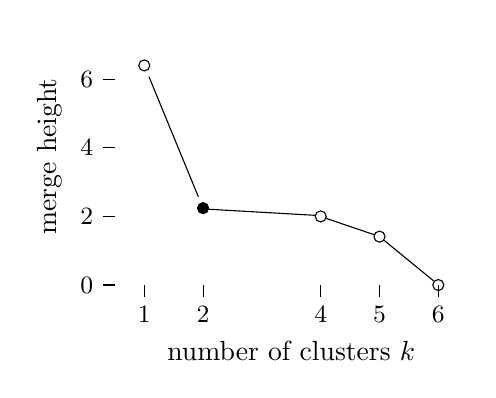
\begin{tikzpicture}
        \begin{axis}[
            xlabel={number of clusters $k$},
            ylabel={merge height},
            xmin=0.5, xmax=6.5,
            ymin=0, ymax=7.5,
            width=0.5\textwidth, height=0.4\textwidth,
            axis line style={draw=none},
            tick style={black, thin},
            xtick={1,2,4,5,6},
            xticklabel style={font=\small},
            yticklabel style={font=\small},
            tick align=outside, tick pos=left,
        ]
        % Elbow point (filled)
        \addplot[only marks, mark=*, mark size=2pt, black] coordinates {(2,2.24)};
        % Other points (open)
        \addplot[only marks, mark=o, mark size=2pt, black] coordinates {(1,6.40) (4,2.00) (5,1.41) (6,0)};
        % Line segments with gaps around each dot
        \draw[black, thin] (axis cs:1.08,6.07) -- (axis cs:1.92,2.57);
        \draw[black, thin] (axis cs:2.08,2.21) -- (axis cs:3.92,2.03);
        \draw[black, thin] (axis cs:4.08,1.95) -- (axis cs:4.92,1.46);
        \draw[black, thin] (axis cs:5.08,1.30) -- (axis cs:5.92,0.12);
        \end{axis}
    \end{tikzpicture}
    \label{fig:hc_elbow}
    \end{figure}


\begin{marginfigure}
    \centering
    \begin{tikzpicture}
        \begin{axis}[
            xmin=-1.8, xmax=5.5, ymin=-5, ymax=105,
            width=\marginparwidth, height=1.8\marginparwidth,
            axis line style={draw=none},
            tick style={black, thin},
            xtick=\empty,
            ytick={1.00, 3.00, 96.6},
            yticklabels={$1.0$, $3.0$, $96.6$},
            yticklabel style={font=\tiny},
            tick align=outside,
            tick pos=left,
        ]
        % Merge 1: x1(0)-x2(1) at h=1.00
        \draw[thick] (axis cs:0,0) -- (axis cs:0,1.00) -- (axis cs:1,1.00) -- (axis cs:1,0);
        % Merge 2: x5(4)-x6(5) at h=2.00
        \draw[thick] (axis cs:4,0) -- (axis cs:4,2.00) -- (axis cs:5,2.00) -- (axis cs:5,0);
        % Merge 3: x4(3) + {x5,x6}(root 4.5,2.00) at h=2.67
        \draw[thick] (axis cs:3,0) -- (axis cs:3,2.67) -- (axis cs:4.5,2.67) -- (axis cs:4.5,2.00);
        % Merge 4: {x1,x2}(root 0.5,1.00) + x3(2) at h=3.00
        \draw[thick] (axis cs:0.5,1.00) -- (axis cs:0.5,3.00) -- (axis cs:2,3.00) -- (axis cs:2,0);
        % Merge 5: {x1-x3}(root 1.25,3.00) + {x4-x6}(root 3.75,2.67) at h=96.6
        \draw[thick] (axis cs:1.25,3.00) -- (axis cs:1.25,96.6) -- (axis cs:3.75,96.6) -- (axis cs:3.75,2.67);
        % Leaf labels
        \node[anchor=north, font=\tiny] at (axis cs:0,-2)  {$x_1$};
        \node[anchor=north, font=\tiny] at (axis cs:1,-2)  {$x_2$};
        \node[anchor=north, font=\tiny] at (axis cs:2,-2)  {$x_3$};
        \node[anchor=north, font=\tiny] at (axis cs:3,-2)  {$x_4$};
        \node[anchor=north, font=\tiny] at (axis cs:4,-2)  {$x_5$};
        \node[anchor=north, font=\tiny] at (axis cs:5,-2)  {$x_6$};
        % Cut line between 3.00 and 96.6
        \draw[densely dashed, black!60] (axis cs:-1.5,50) -- (axis cs:5.3,50);
        \end{axis}
    \end{tikzpicture}
    \caption{Ward's dendrogram on true scale ($\Delta$var). Four merges pack below 3.0; the final merge towers at 96.6. The gap dwarfs the one in the single-linkage dendrogram above.}
    \label{fig:dendrogram_ward}
    \end{marginfigure}

\newthought{Ward's dendrogram} for the same six points is shown alongside.
Heights are no longer Euclidean distances but variance increases\index{Ward's method!variance increase}: each merge height records the rise in total within-cluster variance caused by that merge.


\newthought{Compare the gaps.} Single linkage gave a gap from 2.24 to 6.40 (ratio ${\approx}2.9\times$). 
Ward's gives a gap from 3.00 to 96.6 (ratio ${\approx}32\times$). Ward's tends to amplify the gap signal, 
making cluster number selection more pronounced. 






\vspace{2.5em}
\newthought{How do we infer new data points?}\index{hierarchical clustering!new data} The dendrogram 
is a static structure built on the original data; it does not directly provide 
a way to assign new points to clusters. But, given a cut of the dendrogram into $K$ clusters, 
we can assign a new point $x_{\mathrm{new}}$ to the cluster whose centroid is closest 
under the same distance metric used for clustering. Or we assign it to a cluster based on the closest leaf.


\iffalse
\vspace{2.5em}

\newthought{Excursion: Prim's MST and Single Linkage.}\index{minimum spanning tree}\index{Prim's algorithm}
Single linkage is the one linkage criterion with a fundamentally cheaper algorithm.
The key insight is a duality: the single-linkage dendrogram is equivalent to the minimum spanning tree (MST) of the complete pairwise distance graph.
Sorting the $n-1$ MST edges by weight gives the merge heights of the dendrogram in order.

\newthought{Prim's algorithm}\cite{Prim1957} builds an MST greedily.
It maintains a set $S$ of visited nodes and, for every unvisited node $v$, a value $\delta(v)$ equal to the shortest edge from $v$ to any node already in $S$.

\begin{enumerate}[leftmargin=*, nosep]
    \item Start with any node in $S$; set $\delta(v) \gets d(v, s_0)$ for all $v$.
    \item Repeat $n-1$ times: find $v^* = \arg\min_{v \notin S} \delta(v)$, add $v^*$ to $S$, record edge $(v^*, \mathrm{parent}(v^*))$ with weight $\delta(v^*)$.
    \item Update: for each $v \notin S$, set $\delta(v) \gets \min\bigl(\delta(v),\, d(v, v^*)\bigr)$.
\end{enumerate}

\marginnote{\newthought{Why the duality holds.} At each Prim step, $\delta(v)$ is the single-linkage distance from singleton $\{v\}$ to the current tree cluster $S$: $D_{\mathrm{single}}(\{v\}, S) = \min_{u \in S} d(v, u)$. Selecting $v^*$ is therefore identical to selecting the globally minimal inter-cluster distance, exactly the single-linkage merge criterion.}

Step 2 costs $O(n)$ per iteration (linear scan of $\delta$); step 3 costs $O(n)$ per iteration.
Over $n-1$ iterations the total is $O(n^2)$ time and $O(n)$ space since only the array $\delta$ and a parent pointer per node are needed.
This matches SLINK\index{SLINK}\cite{Sibson1973}, the classical optimal algorithm for single linkage, which encodes the same MST structure via a pointer representation without building the full distance matrix.
\fi

% \vspace{2.5em}
%
% % OPTIONAL: BIRCH deep-dive (comment in to expand)
% \newthought{BIRCH: Hierarchical Clustering at Scale}\index{BIRCH}
%
% \newthought{BIRCH}\cite{Zhang1996} (Balanced Iterative Reducing and Clustering using Hierarchies) breaks the $O(n^2)$ barrier by replacing the raw data points with a compact summary before running hierarchical clustering.
%
% \newthought{The Clustering Feature} (CF)\index{BIRCH!clustering feature} is the core data structure.
% For a set of $n$ points $\{x_1,\ldots,x_n\}$, the CF stores three statistics:
%
% \begin{align*}
%     \mathrm{CF} &= \bigl(n,\;\mathrm{LS},\;\mathrm{SS}\bigr) \\
%     \mathrm{LS} &= \textstyle\sum_{i=1}^{n} x_i \quad \text{(linear sum)} \\
%     \mathrm{SS} &= \textstyle\sum_{i=1}^{n} \|x_i\|^2 \quad \text{(squared sum)}
% \end{align*}
%
% CFs are \textbf{additive}: merging two subsets means adding their triples component-wise, so the centroid and within-cluster variance of any merged group can be recovered without storing individual points.
%
% \marginnote{\newthought{What CF enables.} From $(n,\mathrm{LS},\mathrm{SS})$ alone you can recover the centroid $\mu = \mathrm{LS}/n$, the radius $R = \sqrt{(\mathrm{SS} - \|\mathrm{LS}\|^2/n)\,/\,n}$, and the Ward merge cost between any two CFs: all the quantities hierarchical clustering needs.}
%
% \newthought{The CF-tree}\index{BIRCH!CF-tree} is a height-balanced tree whose leaf nodes each hold the CFs of a small neighbourhood of points.
% BIRCH builds the tree in a \textbf{single pass} over the data: each new point is absorbed into the nearest leaf CF; if the leaf overflows it is split, and splits propagate up exactly as in a B-tree.
% The tree size is controlled by two parameters: the branching factor $B$ and the leaf-entry threshold $T$ (the maximum radius a CF may span).
%
% \newthought{The two-phase algorithm} is:
%
% \begin{enumerate}
%     \item \textbf{Scan.} Read the data once, building the CF-tree. Time $O(n)$, memory $O(\text{tree size}) \ll O(n^2)$.
%     \item \textbf{Cluster.} Apply agglomerative hierarchical clustering to the leaf CFs, not to individual points. If there are $L$ leaves, this costs $O(L^2 \log L)$ with $L \ll n$.
% \end{enumerate}
%
% \marginnote{\newthought{When to use BIRCH.} Use standard agglomerative clustering for $n \leq 10{,}000$. Switch to BIRCH when $n$ grows into the tens or hundreds of thousands. BIRCH is an approximation: points absorbed into the same leaf CF are never separated, so the final clustering can differ from exact Ward's.}
%
% \newthought{The trade-off} is approximation for speed.
% Because entire neighbourhoods are summarised into a single CF, BIRCH cannot recover from an early bad grouping the way exact agglomerative clustering can.
% The threshold $T$ controls the granularity: a tight $T$ keeps more leaf nodes and is more accurate but uses more memory; a loose $T$ compresses aggressively and is faster but coarser.


% ==============================================================================================
% BLOCK 3: STUDENT ACTIVATION
% ==============================================================================================

\newpage

\subsection{Examples \& Exercises}\index{examples}\index{exercises}


% ---------------------------------------------------------------------------
% Exercise 1: By-hand single-linkage (3 points from ch02)
% ---------------------------------------------------------------------------

\begin{marginfigure}
    \centering
    \begin{tikzpicture}
        \begin{axis}[
            xmin=0, xmax=9,
            ymin=0, ymax=9,
            width=\marginparwidth,
            height=\marginparwidth,
            axis line style={draw=none},
            tick style={black, thin},
            xtick={0,3,6,9},
            ytick={0,3,6,9},
            xticklabel style={font=\tiny},
            yticklabel style={font=\tiny},
            tick align=outside,
            tick pos=left,
            xlabel={$x^{(1)}$},
            ylabel={$x^{(2)}$},
        ]
        \addplot[only marks, mark=*, mark size=2pt, black]    coordinates {(1,1)(3,1)};
        \addplot[only marks, mark=*, mark size=2pt, black!55] coordinates {(8,7)};
        % cluster link
        \draw[black!35, thin] (axis cs:1,1) -- (axis cs:3,1);
        \node[font=\small, anchor=south] at (axis cs:1,1) {$x_1$};
        \node[font=\small, anchor=south] at (axis cs:3,1) {$x_2$};
        \node[font=\small, anchor=north] at (axis cs:8,7) {$x_3$};
        \end{axis}
    \end{tikzpicture}
    \caption{The same three points from the K-Means exercise. No centroids this time; the algorithm needs only pairwise distances.}
    \label{fig:hc_exercise_scatter}
\end{marginfigure}

\newthought{Given three points} $x_1{=}(1,1)$, $x_2{=}(3,1)$, $x_3{=}(8,7)$, run 
single-linkage agglomerative clustering step by step.
These are the same points you clustered with K-Means already, but 
this time there is no centroid initialization, no random seed, no choice of $K$.
Your tasks: compute the initial pairwise distance table, 
identify the minimum pair at each step, record each merge, update distances 
using single linkage, and construct the dendrogram.

\marginnote{\newthought{Reuse by design.} Working on the same three points lets you compare the two algorithms directly: K-Means needed an initialization and an iterative loop; hierarchical clustering needs neither.}

\vspace{0.5em}

\newthought{Initial distances.} For each pair $(x_i,\,x_j)$ compute 
the euclidean distance.
With $n{=}3$ there are only $\binom{3}{2}{=}3$ pairs.
Here is the full calculation for $d(x_1,\,x_2)$:

\begin{align*}
    d(x_1,\,x_2) &= \sqrt{(3-1)^2 + (1-1)^2} \\
                 &= \sqrt{4 + 0} \\
                 &= 2
\end{align*}

Compute the remaining two distances yourself, then verify against the table below.
We use symmetries to reduce compute, so only the upper triangle of the distance matrix is filled; 
the diagonal is empty since $d(x_i, x_i) = 0$ is trivial and not needed for merges.

\vspace{2.5em}

\begin{table*}[ht]
\centering
\begin{tabular}{p{0.10\textwidth}p{0.15\textwidth}p{0.15\textwidth}p{0.15\textwidth}}
    \toprule
    & \textbf{$x_1$} & \textbf{$x_2$} & \textbf{$x_3$} \\
    \midrule
    $x_1$ & $-$  & $\mathbf{2.00}$ & $8.49$ \\
    $x_2$ & $-$ & $-$  & $7.81$ \\
    $x_3$ & $-$ & $-$ & $-$ \\
    \bottomrule
\end{tabular}
\vspace{2em}
\caption{Initial pairwise Euclidean distances. The global minimum $d(x_1,x_2){=}2$ (bold) triggers the first merge.}
\label{tab:hc_distances}
\end{table*}

\newthought{First merge.}
The minimum entry is $d(x_1,\,x_2){=}2$.
Merge $x_1$ and $x_2$ into cluster $\{x_1,x_2\}$ at height 2.
Update the distance to the remaining point using single linkage. 
Remember that you do not have to recompute the full distance matrix; 
only the distances to the new cluster $\{x_1,x_2\}$, repurposing the already computed distances 
to $x_1$ and $x_2$ and solving for the minimum:

\begin{align*}
    d\!\left(\{x_1,x_2\},\; x_3\right) &= \min\!\left(d(x_1,x_3),\; d(x_2,x_3)\right) \\
                                        &= \min(8.49,\; 7.81) \\
                                        &= 7.81
\end{align*}

\newthought{Second merge.}
Only two active clusters remain: $\{x_1,x_2\}$ and $\{x_3\}$.
Their distance is 7.81, so they merge at height 7.81.
The dendrogram is complete.

\begin{table*}[ht]
\centering
\begin{tabular}{p{0.05\textwidth}p{0.24\textwidth}p{0.12\textwidth}p{0.40\textwidth}}
    \toprule
    \textbf{Step} & \textbf{Clusters merged} & \textbf{Height} & \textbf{Updated distances (single linkage)} \\
    \midrule
    1 & $x_1,\; x_2$
      & $2.00$
      & $d(\{x_1,x_2\},\,x_3){=}7.81$ \\
    2 & $\{x_1,x_2\},\; x_3$
      & $7.81$
      & Final merge; algorithm complete \\
    \bottomrule
\end{tabular}
\vspace{2em}
\caption{Single-linkage merge history for $x_1, x_2, x_3$. The gap from 2.00 to 7.81 confirms two natural groups, matching the K-Means result from Chapter~2.}
\label{tab:hc_merges}
\end{table*}

% ---------------------------------------------------------------------------
% Exercise 2: Guaranteed termination
% ---------------------------------------------------------------------------

\newthought{Guaranteed termination.}
How many merges did you just perform?
Could there have been more? Fewer? Why?

\newthought{Each merge removes two clusters} from the active set and adds one, 
reducing $|\mathrm{active}|$ by exactly one.
Starting from $n$ singletons, the algorithm reaches $|\mathrm{active}|{=}1$ after 
exactly $n{-}1$ steps. 

\begin{itemize}
    \item For $n{=}3$: exactly 2 merges.
    \item For $n{=}1{,}000$: exactly 999 merges.
\end{itemize}

\marginnote{\newthought{Contrast with K-Means.} K-Means has no guaranteed iteration count. It can converge in 2 iterations or 200, depending on initialization. Hierarchical clustering always finishes in $n{-}1$ steps, with no restarts and no randomness.}

This also means the dendrogram always has $n$ leaves and $n{-}1$ internal nodes.
Verify this on your two-merge trace: 3 leaves, 2 internal nodes, one complete binary tree $T$.


\vspace{2.5em}

% ---------------------------------------------------------------------------
% Exercise 3: Dendrogram reading
% ---------------------------------------------------------------------------
\marginnote{\newthought{Leaf ordering trap.}\index{dendrogram!leaf ordering} A 
dendrogram with $n$ leaves has $2^{n-1}$ valid leaf orderings: 
at each internal node you can swap left and right children without 
changing the hierarchy. Two points adjacent in the plot are not necessarily similar; 
only the merge height tells you when they joined.}

\newthought{Reading the dendrogram.}
Sketch the dendrogram for the three-point trace.
It has two horizontal bars: one at height 2.00 (merging $x_1, x_2$) and one at height 7.81 (merging everything). Now answer the following:
\begin{itemize}
    \item Cut at $h{=}5$. How many clusters do you get? Which points are in each?
    \item Cut at $h{=}1$. How many clusters? What does this tell you?
    \item What is the largest gap between consecutive merge heights? What $K$ does it suggest?
    \item How does the spread of the nodes in the dendrogram relate to an elbow plot over $K$?
\end{itemize}

\newthought{The gap} is $7.81 - 2.00 = 5.81$: the final merge costs nearly four times as 
much as the first. A cut anywhere in this gap yields $K{=}2$ with $C_1{=}\{x_1,x_2\}$, $C_2{=}\{x_3\}$, exactly the partition K-Means found.
% So what is the benefit of the computationally heavier hierarchical clustering if it 
% gives the same result as K-Means?





\vspace{2.5em}

% ---------------------------------------------------------------------------
% Exercise 4: Linkage comparison with chaining
% ---------------------------------------------------------------------------

\newthought{Linkage comparison with chaining.}
Add a bridge point $x_4{=}(5,4)$ to the three points.
This point sits between the two natural groups in a region where no cluster really lives.

\begin{marginfigure}
    \centering
    \begin{tikzpicture}
        \begin{axis}[
            xmin=0, xmax=9,
            ymin=0, ymax=9,
            width=\marginparwidth,
            height=\marginparwidth,
            axis line style={draw=none},
            tick style={black, thin},
            xtick={0,3,6,9},
            ytick={0,3,6,9},
            xticklabel style={font=\tiny},
            yticklabel style={font=\tiny},
            tick align=outside,
            tick pos=left,
            xlabel={$x^{(1)}$},
            ylabel={$x^{(2)}$},
        ]
        \addplot[only marks, mark=*, mark size=2pt, black]    coordinates {(1,1)(3,1)};
        \addplot[only marks, mark=*, mark size=2pt, black!55] coordinates {(8,7)};
        \addplot[only marks, mark=*, mark size=2pt, black!30] coordinates {(5,4)};
        % left cluster link
        \draw[black!35, thin] (axis cs:1,1) -- (axis cs:3,1);
        % chaining bridge
        \draw[black!55, densely dashed] (axis cs:3,1) -- (axis cs:5,4);
        \draw[black!55, densely dashed] (axis cs:5,4) -- (axis cs:8,7);
        \node[font=\small, anchor=south] at (axis cs:1,1) {$x_1$};
        \node[font=\small, anchor=south] at (axis cs:3,1) {$x_2$};
        \node[font=\small, anchor=north] at (axis cs:8,7) {$x_3$};
        \node[font=\small, anchor=south west] at (axis cs:5,4) {$x_4$};
        \end{axis}
    \end{tikzpicture}
    \caption{Bridge point $x_4$ in the gap between the two natural groups. Dashed lines show the chain that single linkage will follow.}
    \label{fig:hc_chaining_exercise}
\end{marginfigure}

Compute the initial $\binom{4}{2}{=}6$ pairwise distances.
Then trace single linkage to completion. Based on our previous trace, 
reuse the distances you already calculated, prior to the merge of $x_1, x_2$ at height 2.00 and 
calculate the missing distances to $x_4$. You should find the second merge of $\{x_1,x_2\}, x_4$ 
at height $\approx 3.61$. Finally merge 
$\{x_1,x_2,x_4\}, x_3$ at height $\approx 4.24$


\newthought{The bridge point} chains the two groups together through nearest-neighbour 
links: $x_2 \to x_4 \to x_3$. What happens with our gap signal? The first merge is 
still $x_1, x_2$ at height 2.00, but the second merge is now $\{x_1,x_2\}, x_4$ at height 3.61 deluting our signal, 
and the final merge is $\{x_1,x_2,x_4\}, x_3$ at height 4.24.

\newthought{Now repeat with complete linkage.}
Replace each $\min$ in the update rule with $\max$.
After step 1 (still $x_1, x_2$ at height 2.00), the updated distance from $\{x_1,x_2\}$ to $x_4$ under complete linkage becomes:

\begin{align*}
    d_{\mathrm{comp}}\!\left(\{x_1,x_2\},\; x_4\right) &= \max\!\left(d(x_1,x_4),\; d(x_2,x_4)\right) \\
                                                          &= \max(5.00,\; 3.61) \\
                                                          &= 5.00
\end{align*}

Check whether $x_4$ still merges with $\{x_1,x_2\}$ next, or whether a different pair is closer.
Trace the remaining merges and compare the complete-linkage dendrogram to the single-linkage one.
Which linkage is more vulnerable to the bridge point? Why?



% ---------------------------------------------------------------------------
% Exercise 5: Why single linkage is fast
% ---------------------------------------------------------------------------

\newthought{Why single linkage is fast.}
Look back at the distance update you performed in the single-linkage trace.
When $C_i$ and $C_j$ merge into $C_m$, the new distance to any remaining cluster $C_k$ is:

\begin{align*}
    D_{\mathrm{single}}(C_m,\, C_k) &= \min\!\bigl(D(C_i,\, C_k),\; D(C_j,\, C_k)\bigr)
\end{align*}

One comparison, two table lookups, no access to the original data points.
The update depends only on values already in the distance matrix.
This means the entire algorithm can run on the $n \times n$ matrix alone; once initialized, the raw data is never touched again.

\marginnote{\newthought{SLINK}\index{SLINK} exploits exactly this property. Because single linkage only needs nearest-neighbour information, the merge sequence is equivalent to a minimum spanning tree. Prim's algorithm builds that tree in $O(n^2)$, matching SLINK's optimal complexity.}

\newthought{Now compare with Ward's update.}
Recall that Ward's distance measures the increase in total within-cluster variance caused by a merge.
For two clusters $C_a$ and $C_b$ with centroids $\mu_a, \mu_b$ and sizes $n_a, n_b$:

\begin{align*}
    D_{\mathrm{Ward}}(C_a,\, C_b) &= \frac{n_a \cdot n_b}{n_a + n_b}\,\|\mu_a - \mu_b\|^2
\end{align*}

To update the distance after a merge, you must recompute the centroid of the merged cluster and then apply the definition again.
This means going back to the raw data, unlike single linkage which never looks beyond the distance matrix.

\marginnote{\newthought{Shortcut.} The Lance-Williams formula\index{Lance-Williams formula} expresses Ward's update purely in terms of existing table entries and cluster sizes, avoiding the detour through centroids. The merge loop still runs in $O(n^2 \log n)$ at best and $O(n^3)$ in the naive implementation, compared to $O(n^2)$ for single linkage.}

\newthought{Verify the difference.}
For the three-point trace, compute the Ward distance update for $D_{\mathrm{Ward}}(\{x_1,x_2\},\, x_3)$ from the definition and confirm that it gives a different value than the single-linkage update.
Ward's initial distance between two singletons reduces to $\tfrac{1}{2}\|x_i - x_j\|^2$.
The first merge is still $x_1, x_2$ (at Ward height $\tfrac{1}{2} \cdot 4 = 2.00$).
After merging, the centroid of $\{x_1, x_2\}$ is $\mu_{12} = (2, 1)$.
Now apply the definition to compute the distance to the remaining singleton $x_3$:

\begin{align*}
    D_{\mathrm{Ward}}\!\left(\{x_1,x_2\},\; x_3\right) &= \frac{n_{12} \cdot n_3}{n_{12} + n_3}\,\|\mu_{12} - x_3\|^2 \\
                                                          &= \frac{2 \cdot 1}{2+1}\,\left\|\begin{pmatrix}2\\1\end{pmatrix} - \begin{pmatrix}8\\7\end{pmatrix}\right\|^2 \\
                                                          &= \frac{2}{3}\left\|\begin{pmatrix}-6\\-6\end{pmatrix}\right\|^2 \\
                                                          &= \frac{2}{3}\bigl((-6)^2 + (-6)^2\bigr) \\
                                                          &= \frac{2}{3}(36 + 36) \\
                                                          &= \frac{2}{3} \cdot 72 \\
                                                          &= 48.00
\end{align*}

Single linkage gave 7.81 (a Euclidean distance); Ward's gives 48.00 (a variance increase).
The numbers are not comparable across linkage criteria, but within each criterion they determine the merge order.

\newthought{Back-of-envelope: scalability.}
The distance matrix stores $\binom{n}{2}$ entries.
For $n{=}50{,}000$ with 64-bit floats, that is $\binom{50000}{2} \times 8 \approx 9.3\;\mathrm{GB}$.
For $n{=}100{,}000$: roughly $37\;\mathrm{GB}$.


\vspace{2.5em}

% ---------------------------------------------------------------------------
% Exercise 6: Coding exercise
% ---------------------------------------------------------------------------

\marginnote{\newthought{Code} will be provided as a Python notebook.
Use it as a starting point, break things, and observe what changes.}

\newthought{back at the coffeetable.}
Same 1\,797 coffee aroma fingerprints, ten brewing methods, two coordinates.
Compute the pairwise distance matrix, implement single, complete, and average 
linkage from scratch, then run all four methods and compare 
the truncated dendrograms.
Cut each tree at $K{=}3$, colour the scatter plot, and compare with $K$-Means at $K{=}3$.

\newthought{What to observe.}
Single linkage chains into one dominant cluster.
Complete and Ward yield balanced partitions; the $K$-Means result most closely 
resembles Ward's, because both favour compact, spherical clusters.
One hierarchical run gives you every $K$ from 1 to $n$.



\vspace{2.5em}

% ---------------------------------------------------------------------------
% Self-reflection, recap, bridge
% ---------------------------------------------------------------------------

\newthought{Self-Reflection and Recap}\index{reflection}\index{recap}

\newthought{Self-Reflection} questions to guide your thinking:
\begin{itemize}
    \item What does the merge height in a dendrogram represent, and why does a large gap between consecutive heights signal a natural number of clusters?
    \item Why does single linkage produce chaining while complete linkage does not? What property of each formula causes this difference?
    \item In what situations would you prefer Ward's linkage over single or complete linkage? When would Ward's fail?
    \item You compute a dendrogram and find that the top-level merge height is only marginally larger than the second-to-top merge height. What does this tell you about the cluster structure?
    \item What is the computational bottleneck of hierarchical clustering, and what approximate methods exist to overcome it at scale?
    \item Why is a bad early merge more damaging in hierarchical clustering than a bad initial assignment in K-Means? What mechanism does K-Means have that the dendrogram lacks?
\end{itemize}

\newthought{Recap} of Key Concepts:
\begin{itemize}
    \item Agglomerative clustering greedily merges the two closest clusters at each step, producing a dendrogram that encodes all flat partitions from $K{=}1$ to $K{=}n$ in a single structure
    \item The algorithm terminates in exactly $n{-}1$ merges; no initialization, no restarts, no convergence check
    \item Ward's linkage minimises the same within-cluster variance as K-Means; a single Ward dendrogram encodes all partitions from $K{=}1$ to $K{=}n$, each equivalent to a K-Means run for that $K$ but without iterative re-assignment, so Ward's inherits the spherical bias and cannot correct it
    \item Single linkage detects elongated clusters but suffers from chaining; complete and Ward's linkage produce compact clusters and are more robust to sparse bridge points
    \item Single linkage is uniquely fast ($O(n^2)$ via SLINK) because its update rule reduces to a single $\min$ over existing table entries, equivalent to a minimum spanning tree
    \item A large gap between consecutive merge heights is the dendrogram signal for a natural number of clusters, analogous to the elbow in K-Means inertia curves
    \item Leaf adjacency in a dendrogram does not imply similarity; only the merge height matters
    \item The $O(n^2)$ distance matrix limits hierarchical clustering to moderate-sized datasets without approximation methods such as BIRCH
\end{itemize}


\marginnote{\newthought{Teaser} How can we define a cluster without any centroid, any
linkage criterion, or any choice of $K$, label outliers as noise automatically, 
and still recover clusters of arbitrary shape?}

\newthought{The root of hierarchical failure.} Every linkage criterion measures 
distance between points or boundaries locally. No criterion has a concept of empty 
space or of sparsity. In the next Chapter we will introduce and leverage the concept 
of density. Starting from the single question that hierarchical clustering cannot answer; 
what are the characteristics of a space or neighbourhood?


\marginnote{\newthought{feedback}}
